\documentclass[11pt,a4paper,titlepage]{article}
\usepackage[utf8]{inputenc}
\usepackage[left=1.5cm,text={18cm, 25cm},top=2.5cm]{geometry}
\usepackage{setspace}
\usepackage{graphicx}
\usepackage[czech]{babel}
\usepackage{caption}
\usepackage{subcaption}
\usepackage{subfig}
\usepackage{float}
\setlength{\parindent}{0cm}
\setlength{\parskip}{1em}
\sloppy

\begin{document}
    \section{Rozbor a analýza výpočtu úrovně vrcholu}
        Účelem algoritmu je určit počet hran na cestě od vrcholu do kořene stromu. Tento počet
        lze určit rozdílem v počtu zpětných a dopředných hran na zbytku Eulerovy cesty od vrcholu
        do uzlu.

        Tento algoritmus pracuje tedy s binárním stromem, kde mezi rodičovským uzlem a potomkem existují
        právě 2 hrany -- dopředná a zpětná. Každá z těchto hran je v algoritmu reprezentována jedním procesem.
        Každý z těchto procesů si určí předchůdce i následníka a tím se vytvoří Eulerova cesta. Dále
        si procesy nastaví výchozí hodnotu váhy na základě toho, zda je proces dopřednou či zpětnou
        hranou. Následuje algoritmus součtu suffixů pro učení výsledné váhy hrany a následná oprava
        výsledku pro určení vzdálenosti uzlu od kořene.

        \subsection{Složitost a cena algoritmu}
        Každý z procesů si dokáže v konstantním čase určit svého předchůdce, následníka i svou počáteční váhu.
        Algoritmus sumy suffixů má složitost $\mathcal{O}(log_2 p)$, kde $p$ je počet procesů. Oprava výsledku
        je provedena opět v konstantním čase.

        Celková časová složitost algoritmu je tedy $\mathcal{O}(log_2 p)$. Počet potřebných procesů k~dosažení této
        časové složitosti je $(n - 1) * 2$. Výsledná cena algoritmu potom bude $\mathcal{O}(n \times log_2 n)$.
        Vzhledem k~časové složitosti sekvenční implementace algoritmu se jedná o~optimální cenu.

	\section{Implementace}
        Aplikace \texttt{vuv} pracuje se stromem zadaným sekvencí znaků jako první parametr aplikace.
        Tyto znaky mohou být libovolné a mohou se libovolně opakovat. Na výstupu aplikace je jejich pořadí zachováno.

        Samotná aplikace \texttt{vuv} tedy přijímá 1 argument reprezentující strom a lze ji spustit například pomocí následujícího příkazu:
\begin{verbatim}
mpirun --prefix /usr/local/share/OpenMPI -np PROCESS_COUNT vuv SEQUENCE
\end{verbatim}
        Při spuštění aplikace je nutné zadat správný počet procesů, jinak aplikace končí s~návratovou hodnotou 2.
        Počet procesů je určen vzorcem $(n - 1)*2$, kde $n$ je nejblížší druhá mocnina délky vstupní sekvence.
        Důvodem této úpravy algoritmu je skutečnost, že implementace aplikace vyžaduje pro správnou funkcionalitu
        vyvážený binární strom. Ve chvíli, kdy je takto navýšen počet procesů, se i uměle navýší délka stromu.
        Informaci o navýšení délky stromu nese pouze kořenový proces, který následně přidané uzly ignoruje
        během výpisu výsledných vzdáleností uzlů od kořenu.

	\section{Komunikace}
        Komunikaci začíná kořenový proces odesláním velikosti stromu všem procesům. Na základě této velikosti stromu a ID procesu si každý
        proces určí zdrojový a cílový uzel (proces je orientovanou hranou mezi těmito uzly). Následně si na základě těchto uzlů, svého ID
        a délky stromu určí i následníka a předchůdce. Následuje algoritmus součtu suffixů, kde proces v iteracích odesílá svým sousedům
        svou váhu, následníka a předchůdce a zároveň tyto hodnoty přijímá a aktualizuje si své sousedy a svou aktuální váhu. Poté, co proces
        nemá žádné sousedy, odešle index zdrojového uzlu a svou váhu (jedná se již o upravenou váhu) procesu s ID 0.

        \begin{figure}[H]
            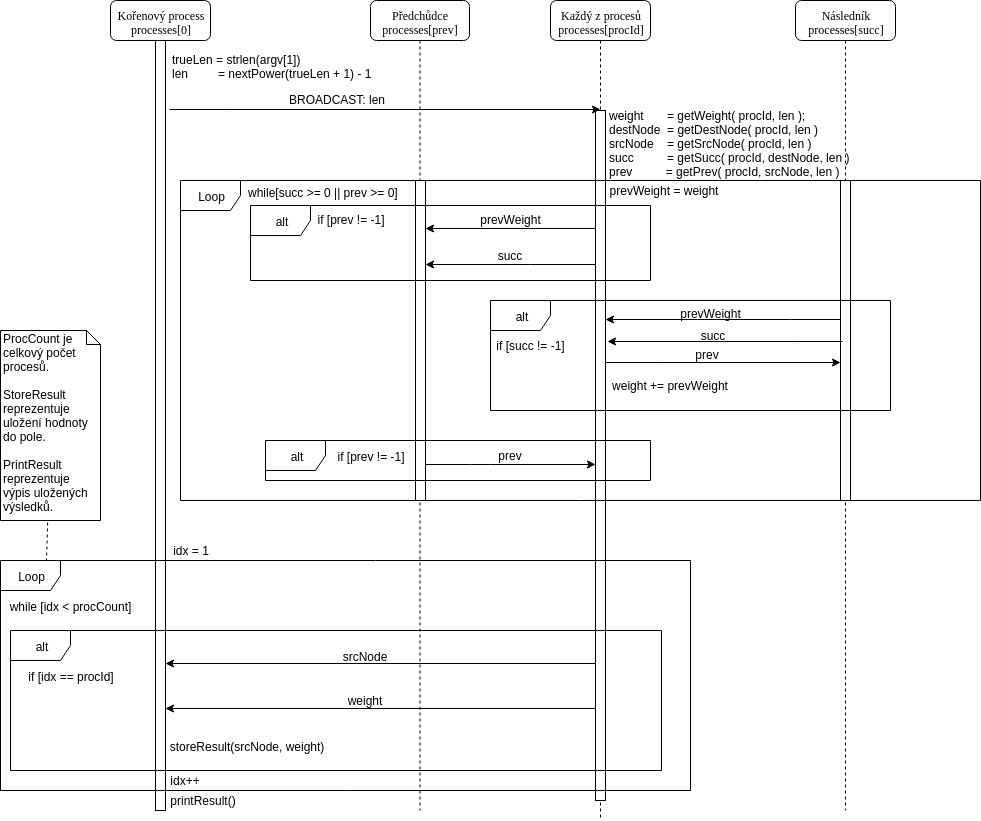
\includegraphics[width=1\linewidth]{sequenceDiagram.png}
            \caption{Komunikace mezi procesy}
        \end{figure}

	\section{Závěr}
        Protože si každý proces dovede určit svou výchozí váhu, předchůdce, následníka, počáteční a cílový uzel konstantní složitostí,
        a protože implementace algoritmu sumy suffixů má složitost $\mathcal{O}(\log_2 n)$, odpovídá výsledná časová složitost
        aplikace výsledkům analýzy v úvodu. Následná oprava výsledku má též konstantní časovou složitost a na výslednou třídu složitosti
        algoritmu tedy nemá žádný vliv.

\end{document}
